% WAEC General Mathematics Lecture Notes
% Topic: Bearings, Angles of Elevation/Depression, Longitude and Latitude
% Paper Size: Ledger (11in x 17in)

\documentclass[10pt]{article}
\usepackage[landscape,paperwidth=17in,paperheight=11in,margin=0.6in]{geometry}
\usepackage{amsmath,amssymb,amsthm}
\usepackage{multicol}
\usepackage{enumitem}
\usepackage{fancyhdr}
\usepackage{graphicx}
\usepackage{tcolorbox}
\usepackage{xcolor}
\usepackage{tikz}
\usepackage{array}
\usepackage{booktabs}

\usetikzlibrary{shapes,arrows,positioning,calc,angles,quotes,decorations.markings}

% Define custom colors
\definecolor{primaryblue}{RGB}{0,102,204}
\definecolor{secondarygreen}{RGB}{0,153,76}
\definecolor{warningred}{RGB}{204,0,0}
\definecolor{exampleorange}{RGB}{255,140,0}
\definecolor{purplemath}{RGB}{102,0,153}

% Custom theorem environments
\theoremstyle{definition}
\newtheorem{definition}{Definition}[section]
\newtheorem{theorem}{Theorem}[section]
\newtheorem{example}{Example}[section]
\newtheorem{exercise}{Exercise}[section]

% Custom boxes
\newtcolorbox{keypoint}{colback=primaryblue!5,colframe=primaryblue,title=Key Point}
\newtcolorbox{formulabox}{colback=secondarygreen!5,colframe=secondarygreen,title=Important Formula}
\newtcolorbox{warningbox}{colback=warningred!5,colframe=warningred,title=Common Mistake}
\newtcolorbox{examplebox}{colback=exampleorange!5,colframe=exampleorange,title=Worked Example}

% Header and Footer
\pagestyle{fancy}
\fancyhf{}
\lhead{\textbf{WAEC General Mathematics}}
\chead{\textbf{Bearings, Angles \& Coordinates}}
\rhead{\textbf{Lecture Notes}}
\cfoot{\thepage}
\setlength{\headheight}{14pt}

\title{\Huge\bfseries Bearings and Distances\\
Angles of Elevation \& Depression\\
Longitude and Latitude\\[0.3cm]
\Large WAEC General Mathematics Comprehensive Lecture Notes}
\author{Academic Lecture Series}
\date{}

\begin{document}

\maketitle
\thispagestyle{fancy}

\begin{multicols}{2}

\section{Bearings and Distances}

\subsection{Introduction to Bearings}

\begin{definition}
A \textbf{bearing} is the direction or path along which something moves or along which it points, measured as an angle from a reference direction (usually North).
\end{definition}

\subsection{Types of Bearings}

\begin{definition}
\textbf{1. Compass Bearings (Cardinal Points):}
\begin{itemize}
\item Use cardinal directions: N, S, E, W
\item Measured as angles from North or South
\item Format: N$\theta$°E, S$\theta$°W, etc.
\item Examples: N30°E, S45°W, N60°W
\end{itemize}

\textbf{2. Three-Figure Bearings (True Bearings):}
\begin{itemize}
\item Measured clockwise from North
\item Always use three digits (000° to 360°)
\item Format: $\theta$°
\item Examples: 045°, 135°, 270°
\end{itemize}
\end{definition}

\begin{keypoint}
\textbf{Cardinal Directions:}
\begin{itemize}
\item North (N) = 000° or 360°
\item East (E) = 090°
\item South (S) = 180°
\item West (W) = 270°
\end{itemize}
\end{keypoint}

\subsection{Converting Between Bearing Types}

\begin{examplebox}
\textbf{Example 1.1:} Convert the following compass bearings to three-figure bearings:
\begin{enumerate}[label=(\alph*)]
\item N30°E
\item S45°W
\item N60°W
\item S25°E
\end{enumerate}

\textbf{Solution:}

\begin{center}
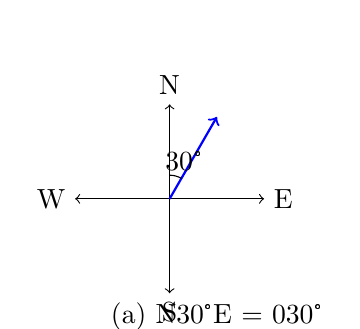
\begin{tikzpicture}[scale=0.6]
% N30°E
\draw[->] (0,0) -- (0,2) node[above] {N};
\draw[->] (0,0) -- (2,0) node[right] {E};
\draw[->] (0,0) -- (0,-2) node[below] {S};
\draw[->] (0,0) -- (-2,0) node[left] {W};
\draw[->,thick,blue] (0,0) -- (1,1.732);
\draw (0,0.5) arc (90:60:0.5);
\node at (0.3,0.8) {30°};
\node at (1,-2.5) {(a) N30°E = 030°};
\end{tikzpicture}
\quad
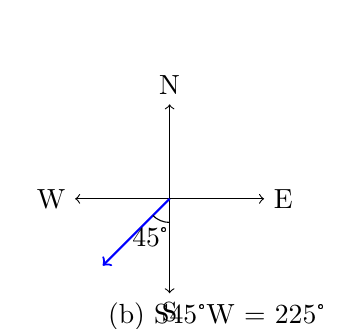
\begin{tikzpicture}[scale=0.6]
% S45°W
\draw[->] (0,0) -- (0,2) node[above] {N};
\draw[->] (0,0) -- (2,0) node[right] {E};
\draw[->] (0,0) -- (0,-2) node[below] {S};
\draw[->] (0,0) -- (-2,0) node[left] {W};
\draw[->,thick,blue] (0,0) -- (-1.414,-1.414);
\draw (0,-0.5) arc (270:225:0.5);
\node at (-0.4,-0.8) {45°};
\node at (1,-2.5) {(b) S45°W = 225°};
\end{tikzpicture}
\end{center}

\textbf{(a)} N30°E: Start from North (000°), go 30° clockwise (towards East)
\[= 030°\]

\textbf{(b)} S45°W: Start from South (180°), go 45° clockwise (towards West)
\[= 180° + 45° = 225°\]

\textbf{(c)} N60°W: Start from North (000°), go 60° anticlockwise (or 360° - 60°)
\[= 360° - 60° = 300°\]

\textbf{(d)} S25°E: Start from South (180°), go 25° anticlockwise (or 180° - 25°)
\[= 180° - 25° = 155°\]
\end{examplebox}

\begin{examplebox}
\textbf{Example 1.2:} Convert 135° to compass bearing.

\textbf{Solution:}
135° is between 090° (East) and 180° (South).

Angle from South = 180° - 135° = 45°

Since it's east of south: \textbf{S45°E}
\end{examplebox}

\subsection{Back Bearings}

\begin{definition}
The \textbf{back bearing} is the bearing from point B to point A when the bearing from A to B is known.

\textbf{Rule:}
\begin{itemize}
\item If bearing $< 180°$: Back bearing = Bearing + 180°
\item If bearing $\geq 180°$: Back bearing = Bearing - 180°
\end{itemize}

Or simply: Back bearing = (Bearing + 180°) mod 360°
\end{definition}

\begin{examplebox}
\textbf{Example 1.3:} Find the back bearings:
\begin{enumerate}[label=(\alph*)]
\item Bearing of B from A is 065°
\item Bearing of Q from P is 245°
\end{enumerate}

\textbf{Solution:}

\textbf{(a)} 065° + 180° = 245°
\newline Bearing of A from B = 245°

\textbf{(b)} 245° - 180° = 065°
\newline Bearing of P from Q = 065°
\end{examplebox}

\subsection{Distance and Bearing Problems}

\begin{examplebox}
\textbf{Example 1.4:} A ship sails 50 km on a bearing of 060° from port A to point B. It then sails 80 km on a bearing of 150° to point C.
\begin{enumerate}[label=(\alph*)]
\item Sketch the path
\item Find the distance AC
\item Find the bearing of C from A
\end{enumerate}

\textbf{Solution:}

\textbf{(a)} 
\begin{center}
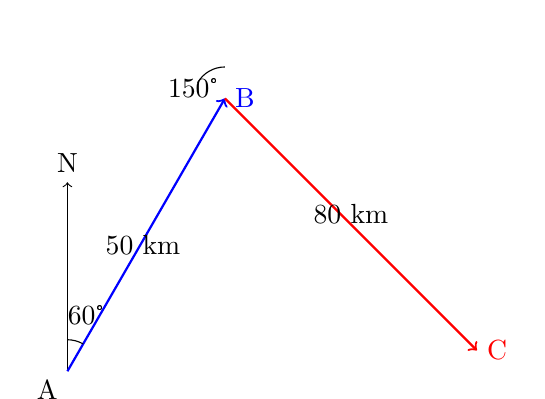
\begin{tikzpicture}[scale=0.8]
\draw[->] (0,0) -- (0,3) node[above] {N};
\draw[->,thick,blue] (0,0) -- (2.5,4.33) node[right] {B};
\draw[->,thick,red] (2.5,4.33) -- (6.5,0.33) node[right] {C};
\node at (0,0) [below left] {A};
\draw (0,0.5) arc (90:60:0.5);
\node at (0.3,0.9) {60°};
\node at (1.2,2) {50 km};
\draw (2.5,4.83) arc (90:150:0.5);
\node at (2,4.5) {150°};
\node at (4.5,2.5) {80 km};
\end{tikzpicture}
\end{center}

\textbf{(b)} Using the angle at B:
\begin{itemize}
\item Bearing from A to B = 060°
\item Bearing from B to C = 150°
\item Angle ABC = 150° - 60° = 90°
\end{itemize}

Since angle at B is 90°, use Pythagoras:
\begin{align*}
AC^2 &= AB^2 + BC^2\\
&= 50^2 + 80^2\\
&= 2500 + 6400\\
&= 8900\\
AC &= \sqrt{8900}\\
&= 94.3 \text{ km}
\end{align*}

\textbf{(c)} Find angle CAB using trigonometry:
\begin{align*}
\tan(\text{angle CAB}) &= \frac{BC}{AB} = \frac{80}{50} = 1.6\\
\text{angle CAB} &= \tan^{-1}(1.6) = 58°
\end{align*}

Bearing of C from A = 060° + 58° = 118°
\end{examplebox}

\begin{examplebox}
\textbf{Example 1.5:} Town B is 100 km from town A on a bearing of 120°. Town C is 80 km from A on a bearing of 200°. Find the distance BC.

\textbf{Solution:}

\begin{center}
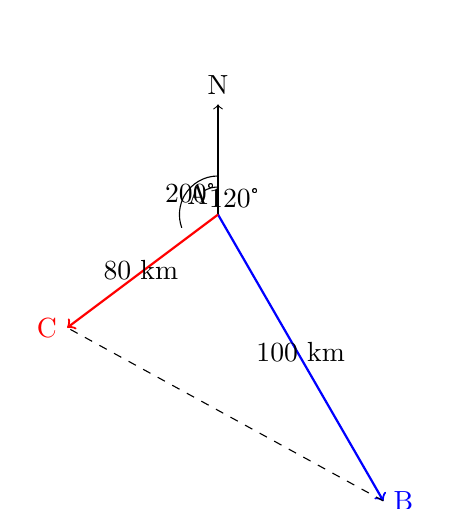
\begin{tikzpicture}[scale=0.7]
\coordinate (A) at (0,0);
\coordinate (B) at (3,-5.196);
\coordinate (C) at (-2.736,-2.052);
\draw[->] (0,0) -- (0,2) node[above] {N};
\draw[->,thick,blue] (A) -- (B) node[right] {B};
\draw[->,thick,red] (A) -- (C) node[left] {C};
\draw[dashed] (B) -- (C);
\node at (A) [above left] {A};
\node at (1.5,-2.5) {100 km};
\node at (-1.4,-1) {80 km};
\draw (0,0.5) arc (90:120:0.5);
\draw (0,0.7) arc (90:200:0.7);
\node at (0.3,0.3) {120°};
\node at (-0.5,0.4) {200°};
\end{tikzpicture}
\end{center}

Angle BAC = 200° - 120° = 80°

Using cosine rule:
\begin{align*}
BC^2 &= AB^2 + AC^2 - 2(AB)(AC)\cos(80°)\\
&= 100^2 + 80^2 - 2(100)(80)\cos(80°)\\
&= 10000 + 6400 - 16000(0.1736)\\
&= 16400 - 2777.6\\
&= 13622.4\\
BC &= 116.7 \text{ km}
\end{align*}
\end{examplebox}

\section{Angles of Elevation and Depression}

\subsection{Definitions}

\begin{definition}
\textbf{Angle of Elevation:} The angle between the horizontal line of sight and the line of sight upward to an object above the horizontal.

\textbf{Angle of Depression:} The angle between the horizontal line of sight and the line of sight downward to an object below the horizontal.
\end{definition}

\begin{center}
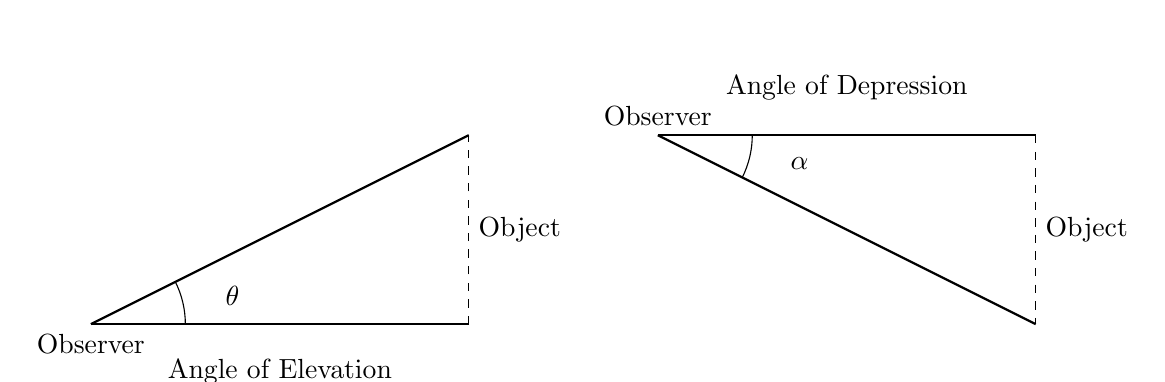
\begin{tikzpicture}[scale=1.2]
% Angle of elevation
\draw[thick] (0,0) -- (4,0);
\draw[thick] (0,0) -- (4,2);
\draw[dashed] (4,0) -- (4,2);
\draw (1,0) arc (0:26.57:1);
\node at (1.5,0.3) {$\theta$};
\node at (4,1) [right] {Object};
\node at (0,0) [below] {Observer};
\node at (2,-0.5) {Angle of Elevation};

% Angle of depression
\begin{scope}[shift={(6,2)}]
\draw[thick] (0,0) -- (4,0);
\draw[thick] (0,0) -- (4,-2);
\draw[dashed] (4,0) -- (4,-2);
\draw (1,0) arc (0:-26.57:1);
\node at (1.5,-0.3) {$\alpha$};
\node at (4,-1) [right] {Object};
\node at (0,0) [above] {Observer};
\node at (2,0.5) {Angle of Depression};
\end{scope}
\end{tikzpicture}
\end{center}

\begin{keypoint}
If you are looking UP at something, it's an angle of elevation.
\newline If you are looking DOWN at something, it's an angle of depression.

The angle of elevation from point A to B equals the angle of depression from B to A (alternate angles).
\end{keypoint}

\subsection{Solving Elevation/Depression Problems}

\begin{examplebox}
\textbf{Example 2.1:} A man standing 50 m from the base of a building observes that the angle of elevation to the top is 40°. Find the height of the building.

\textbf{Solution:}

\begin{center}
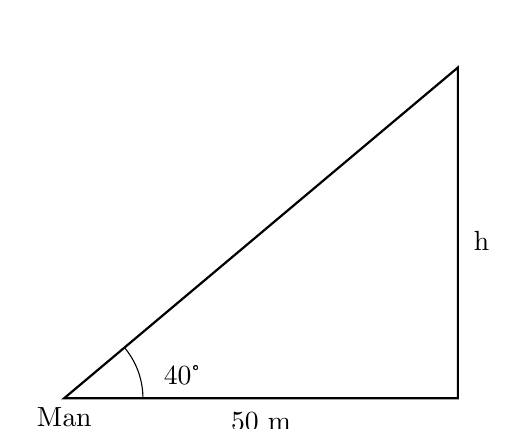
\begin{tikzpicture}[scale=1]
\draw[thick] (0,0) -- (5,0) -- (5,4.2) -- cycle;
\draw[dashed] (5,0) -- (5,4.2);
\draw (1,0) arc (0:40:1);
\node at (1.5,0.3) {40°};
\node at (2.5,-0.3) {50 m};
\node at (5.3,2) {h};
\node at (0,0) [below] {Man};
\end{tikzpicture}
\end{center}

Using trigonometry:
\begin{align*}
\tan(40°) &= \frac{h}{50}\\
h &= 50 \times \tan(40°)\\
&= 50 \times 0.839\\
&= 41.95 \text{ m}
\end{align*}

The building is approximately 42 m tall.
\end{examplebox}

\begin{examplebox}
\textbf{Example 2.2:} From the top of a cliff 80 m high, the angle of depression to a boat at sea is 25°. How far is the boat from the base of the cliff?

\textbf{Solution:}

\begin{center}
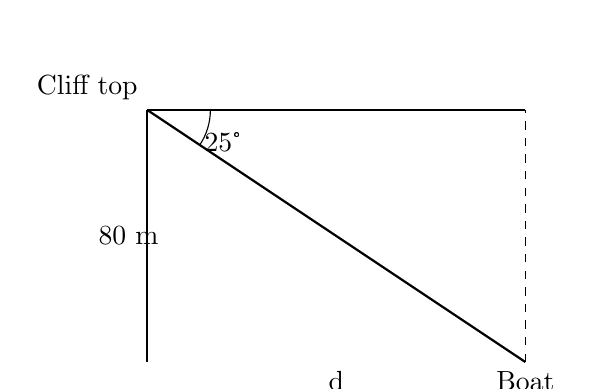
\begin{tikzpicture}[scale=0.8]
\draw[thick] (0,0) -- (0,4);
\draw[thick] (0,4) -- (6,4);
\draw[thick] (0,4) -- (6,0);
\draw[dashed] (6,0) -- (6,4);
\draw (1,4) arc (0:-33.69:1);
\node at (1.2,3.5) {25°};
\node at (-0.3,2) {80 m};
\node at (3,-0.3) {d};
\node at (0,4) [above left] {Cliff top};
\node at (6,0) [below] {Boat};
\end{tikzpicture}
\end{center}

Angle of depression = 25° (from horizontal)
\newline Angle at boat = 25° (alternate angles)

Using trigonometry:
\begin{align*}
\tan(25°) &= \frac{80}{d}\\
d &= \frac{80}{\tan(25°)}\\
&= \frac{80}{0.466}\\
&= 171.7 \text{ m}
\end{align*}

The boat is approximately 172 m from the cliff base.
\end{examplebox}

\begin{examplebox}
\textbf{Example 2.3:} A ladder 10 m long leans against a wall. The angle of elevation of the ladder is 60°. How high up the wall does the ladder reach?

\textbf{Solution:}

\begin{center}
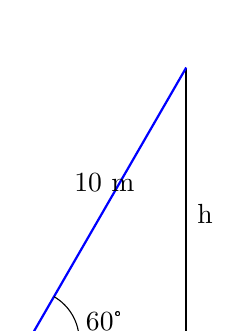
\begin{tikzpicture}[scale=0.8]
\draw[thick] (0,0) -- (2.5,0);
\draw[thick] (2.5,0) -- (2.5,4.33);
\draw[thick,blue] (0,0) -- (2.5,4.33);
\draw (0.8,0) arc (0:60:0.8);
\node at (1.2,0.3) {60°};
\node at (1.2,2.5) {10 m};
\node at (2.8,2) {h};
\end{tikzpicture}
\end{center}

Using trigonometry:
\begin{align*}
\sin(60°) &= \frac{h}{10}\\
h &= 10 \times \sin(60°)\\
&= 10 \times 0.866\\
&= 8.66 \text{ m}
\end{align*}

The ladder reaches approximately 8.7 m up the wall.
\end{examplebox}

\subsection{Combined Problems}

\begin{examplebox}
\textbf{Example 2.4:} From a point on level ground 100 m from the base of a tower, the angle of elevation to the top of the tower is 35°. From a point 50 m closer to the tower, what is the angle of elevation?

\textbf{Solution:}

First find the height of the tower:
\begin{align*}
\tan(35°) &= \frac{h}{100}\\
h &= 100 \times \tan(35°)\\
&= 100 \times 0.700\\
&= 70 \text{ m}
\end{align*}

Now from 50 m away:
\begin{align*}
\tan(\theta) &= \frac{70}{50}\\
&= 1.4\\
\theta &= \tan^{-1}(1.4)\\
&= 54.5°
\end{align*}

The angle of elevation from 50 m is approximately 55°.
\end{examplebox}

\columnbreak

\section{Longitude and Latitude}

\subsection{Basic Concepts}

\begin{definition}
\textbf{Latitude:} Angular distance north or south of the equator, measured in degrees (0° to 90°).
\begin{itemize}
\item North of equator: N latitude (0° to 90°N)
\item South of equator: S latitude (0° to 90°S)
\item Equator: 0° latitude
\end{itemize}

\textbf{Longitude:} Angular distance east or west of the Prime Meridian (Greenwich), measured in degrees (0° to 180°).
\begin{itemize}
\item East of Prime Meridian: E longitude (0° to 180°E)
\item West of Prime Meridian: W longitude (0° to 180°W)
\item Prime Meridian: 0° longitude
\end{itemize}
\end{definition}

\begin{keypoint}
\textbf{Important Facts:}
\begin{itemize}
\item Radius of Earth $\approx$ 6400 km (or 3440 nautical miles)
\item Circumference of Earth $\approx$ 40,000 km
\item 1° of arc on a great circle = $\frac{40000}{360}$ km $\approx$ 111 km
\item Lines of latitude are circles parallel to equator
\item Lines of longitude are semicircles (meridians) from pole to pole
\item All meridians are great circles
\item Only the equator is a great circle among latitudes
\end{itemize}
\end{keypoint}

\subsection{Distance Along Lines of Latitude}

\begin{formulabox}
\textbf{Distance between two points on the same latitude:}

If two points P and Q are on latitude $\theta$° with longitudes $\lambda_1$ and $\lambda_2$:

\textbf{1. Difference in longitude:}
\[\Delta \lambda = |\lambda_2 - \lambda_1|\]

\textbf{2. Radius at latitude $\theta$:}
\[r = R\cos(\theta)\]
where $R$ = radius of Earth

\textbf{3. Distance PQ:}
\[d = \frac{2\pi r \times \Delta\lambda}{360} = \frac{2\pi R\cos(\theta) \times \Delta\lambda}{360}\]

Or: $d = 111 \times \cos(\theta) \times \Delta\lambda$ km
\end{formulabox}

\begin{examplebox}
\textbf{Example 3.1:} Find the distance between two points A(60°N, 30°W) and B(60°N, 50°E) measured along their circle of latitude. (Take $R = 6400$ km, $\pi = \frac{22}{7}$)

\textbf{Solution:}

Both points are on latitude 60°N

Difference in longitude:
\begin{align*}
\Delta\lambda &= 30° + 50° = 80°
\end{align*}

(Add because one is W and one is E)

Radius at 60°N:
\begin{align*}
r &= R\cos(60°)\\
&= 6400 \times 0.5\\
&= 3200 \text{ km}
\end{align*}

Distance:
\begin{align*}
d &= \frac{2\pi r \times 80}{360}\\
&= \frac{2 \times \frac{22}{7} \times 3200 \times 80}{360}\\
&= \frac{1126400}{2520}\\
&= 4470.5 \text{ km}
\end{align*}
\end{examplebox}

\subsection{Distance Along Lines of Longitude}

\begin{formulabox}
\textbf{Distance along a meridian (same longitude):}

If two points P and Q have the same longitude with latitudes $\phi_1$ and $\phi_2$:

\textbf{Difference in latitude:}
\[\Delta\phi = |\phi_2 - \phi_1|\]

\textbf{Distance:}
\[d = \frac{2\pi R \times \Delta\phi}{360} = \frac{\pi R \times \Delta\phi}{180}\]

Or: $d = 111 \times \Delta\phi$ km
\end{formulabox}

\begin{examplebox}
\textbf{Example 3.2:} Find the distance between P(30°N, 40°E) and Q(50°S, 40°E). (Take Earth's radius = 6400 km)

\textbf{Solution:}

Same longitude (40°E), so distance is along a meridian.

Difference in latitude:
\begin{align*}
\Delta\phi &= 30° + 50° = 80°
\end{align*}

(Add because one is N and one is S)

Distance:
\begin{align*}
d &= \frac{2\pi R \times 80}{360}\\
&= \frac{2 \times \frac{22}{7} \times 6400 \times 80}{360}\\
&= \frac{2252800}{2520}\\
&= 8940.5 \text{ km}
\end{align*}

Or using: $d = 111 \times 80 = 8880$ km
\end{examplebox}

\subsection{Shortest Distance (Great Circle Route)}

\begin{formulabox}
\textbf{Shortest distance between two points on Earth's surface:}

The shortest distance is along a great circle. For two points on the same meridian or on the equator, the great circle route is along that line.

For general points, use spherical geometry formulas (typically beyond WAEC scope, but students should know the concept).
\end{formulabox}

\subsection{Position of Places}

\begin{examplebox}
\textbf{Example 3.3:} A plane flies due north from point A(20°N, 15°E) through a distance of 2220 km. Find the position of the final point B.

\textbf{Solution:}

Flying due north means longitude remains constant at 15°E.

Distance = 2220 km

Change in latitude:
\begin{align*}
\Delta\phi &= \frac{2220}{111}\\
&= 20°
\end{align*}

New latitude:
\begin{align*}
\text{Latitude of B} &= 20°N + 20°\\
&= 40°N
\end{align*}

Therefore: B is at (40°N, 15°E)
\end{examplebox}

\begin{examplebox}
\textbf{Example 3.4:} Two towns P and Q are both on latitude 52°N. Their longitudes are 30°W and 70°W respectively. Calculate the distance between P and Q along their circle of latitude. (Take $R = 6400$ km, $\pi = 3.142$)

\textbf{Solution:}

Both on latitude 52°N

Difference in longitude:
\[\Delta\lambda = 70° - 30° = 40°\]

Radius at 52°N:
\begin{align*}
r &= 6400 \times \cos(52°)\\
&= 6400 \times 0.6157\\
&= 3940.5 \text{ km}
\end{align*}

Distance:
\begin{align*}
d &= \frac{2\pi r \times 40}{360}\\
&= \frac{2 \times 3.142 \times 3940.5 \times 40}{360}\\
&= \frac{987732.8}{360}\\
&= 2743.7 \text{ km}
\end{align*}
\end{examplebox}

\subsection{Time Zones}

\begin{keypoint}
\textbf{Time and Longitude:}
\begin{itemize}
\item Earth rotates 360° in 24 hours
\item Therefore: 15° of longitude = 1 hour
\item Or: 1° of longitude = 4 minutes
\item Moving east: time increases
\item Moving west: time decreases
\end{itemize}
\end{keypoint}

\begin{examplebox}
\textbf{Example 3.5:} When it is 12:00 noon at town A(30°E), what is the time at town B(75°E)?

\textbf{Solution:}

Difference in longitude:
\[\Delta\lambda = 75° - 30° = 45°\]

Time difference:
\[\text{Time} = 45° \times 4 \text{ min} = 180 \text{ min} = 3 \text{ hours}\]

Since B is east of A, time at B is ahead:
\[\text{Time at B} = 12:00 + 3:00 = 15:00 \text{ (3:00 PM)}\]
\end{examplebox}

\begin{examplebox}
\textbf{Example 3.6:} A plane leaves town P(15°W) at 9:00 AM and arrives at town Q(45°E) at 5:00 PM the same day. If the plane flew at an average speed of 800 km/h, calculate:
\begin{enumerate}[label=(\alph*)]
\item The time difference between P and Q
\item The actual flight time
\item The distance covered
\end{enumerate}

\textbf{Solution:}

\textbf{(a)} Difference in longitude:
\[\Delta\lambda = 15° + 45° = 60°\]

Time difference:
\[\text{Time} = 60° \times 4 \text{ min} = 240 \text{ min} = 4 \text{ hours}\]

\textbf{(b)} Departure time at P: 9:00 AM
\newline Arrival time at Q: 5:00 PM = 17:00
\newline Time elapsed: 17:00 - 9:00 = 8 hours

But Q is 4 hours ahead of P, so:
\[\text{Actual flight time} = 8 - 4 = 4 \text{ hours}\]

\textbf{(c)} Distance:
\begin{align*}
d &= \text{speed} \times \text{time}\\
&= 800 \times 4\\
&= 3200 \text{ km}
\end{align*}
\end{examplebox}

\section{Practice Exercises}

\subsection{Bearings and Distances}

\begin{exercise}
Convert the following to three-figure bearings:
\begin{enumerate}[label=(\alph*)]
\item N45°E
\item S30°W
\item N70°W
\item S15°E
\end{enumerate}
\end{exercise}

\begin{exercise}
The bearing of B from A is 125°. Find the bearing of A from B.
\end{exercise}

\begin{exercise}
A ship sails 60 km on a bearing of 040° from port P to point Q. It then sails 80 km on a bearing of 130° to point R.
\begin{enumerate}[label=(\alph*)]
\item Find the angle PQR
\item Calculate the distance PR
\end{enumerate}
\end{exercise}

\subsection{Angles of Elevation and Depression}

\begin{exercise}
From a point 80 m from the foot of a tower, the angle of elevation to the top is 38°. Calculate the height of the tower.
\end{exercise}

\begin{exercise}
From the top of a lighthouse 50 m high, the angle of depression to a ship is 15°. How far is the ship from the base of the lighthouse?
\end{exercise}

\begin{exercise}
A 12 m ladder leans against a wall making an angle of 65° with the ground. How high up the wall does it reach?
\end{exercise}

\subsection{Longitude and Latitude}

\begin{exercise}
Calculate the distance along the parallel of latitude 40°N between two points with longitudes 20°E and 65°E. (Take $R = 6400$ km)
\end{exercise}

\begin{exercise}
Find the distance along a meridian between points at 25°N and 45°S. (Use 111 km per degree)
\end{exercise}

\begin{exercise}
When it is 10:00 AM at place A(30°W), what time is it at place B(60°E)?
\end{exercise}

\section{Solutions to Selected Exercises}

\textbf{Solution to Exercise 1:}
\begin{enumerate}[label=(\alph*)]
\item N45°E = 045°
\item S30°W = 180° + 30° = 210°
\item N70°W = 360° - 70° = 290°
\item S15°E = 180° - 15° = 165°
\end{enumerate}

\textbf{Solution to Exercise 2:}
\begin{align*}
\text{Back bearing} &= 125° + 180°\\
&= 305°
\end{align*}

\textbf{Solution to Exercise 3(a):}
Angle at Q = 130° - 40° = 90°

\textbf{Solution to Exercise 3(b):}
Since angle = 90°:
\begin{align*}
PR^2 &= 60^2 + 80^2\\
&= 3600 + 6400\\
&= 10000\\
PR &= 100 \text{ km}
\end{align*}

\textbf{Solution to Exercise 4:}
\begin{align*}
\tan(38°) &= \frac{h}{80}\\
h &= 80 \times \tan(38°)\\
&= 80 \times 0.781\\
&= 62.5 \text{ m}
\end{align*}

\textbf{Solution to Exercise 5:}
\begin{align*}
\tan(15°) &= \frac{50}{d}\\
d &= \frac{50}{\tan(15°)}\\
&= \frac{50}{0.268}\\
&= 186.6 \text{ m}
\end{align*}

\textbf{Solution to Exercise 6:}
\begin{align*}
\sin(65°) &= \frac{h}{12}\\
h &= 12 \times \sin(65°)\\
&= 12 \times 0.906\\
&= 10.9 \text{ m}
\end{align*}

\textbf{Solution to Exercise 7:}
\begin{align*}
\Delta\lambda &= 65° - 20° = 45°\\
r &= 6400 \times \cos(40°)\\
&= 6400 \times 0.766\\
&= 4902.4 \text{ km}\\
d &= \frac{2\pi r \times 45}{360}\\
&= \frac{2 \times 3.142 \times 4902.4 \times 45}{360}\\
&= 3864.5 \text{ km}
\end{align*}

\textbf{Solution to Exercise 8:}
\begin{align*}
\Delta\phi &= 25° + 45° = 70°\\
d &= 111 \times 70\\
&= 7770 \text{ km}
\end{align*}

\textbf{Solution to Exercise 9:}
\begin{align*}
\Delta\lambda &= 30° + 60° = 90°\\
\text{Time difference} &= 90° \times 4 \text{ min}\\
&= 360 \text{ min} = 6 \text{ hours}\\
\text{Time at B} &= 10:00 + 6:00\\
&= 16:00 \text{ (4:00 PM)}
\end{align*}

\section{Summary of Key Formulas}

\begin{formulabox}
\textbf{Bearings:}
\begin{itemize}
\item Back bearing = Bearing $\pm$ 180°
\item Use cosine/sine rules for distances
\end{itemize}

\textbf{Angles of Elevation/Depression:}
\begin{align*}
\tan(\theta) &= \frac{\text{opposite}}{\text{adjacent}}\\
\sin(\theta) &= \frac{\text{opposite}}{\text{hypotenuse}}\\
\cos(\theta) &= \frac{\text{adjacent}}{\text{hypotenuse}}
\end{align*}

\textbf{Longitude and Latitude:}
\begin{align*}
\text{Along latitude: } d &= 111 \times \cos(\phi) \times \Delta\lambda \text{ km}\\
\text{Along longitude: } d &= 111 \times \Delta\phi \text{ km}\\
\text{Time difference} &= \Delta\lambda \times 4 \text{ minutes}
\end{align*}
\end{formulabox}

\section{Examination Tips}

\begin{tcolorbox}[colback=blue!5,colframe=blue!75!black,title=Strategy for WAEC Exams]

\textbf{Bearings:}
\begin{enumerate}
\item Always draw diagrams
\item Mark North direction at each point
\item Use appropriate triangle rules
\item Check if angles are at the correct vertex
\end{enumerate}

\textbf{Elevation/Depression:}
\begin{enumerate}
\item Draw right-angled triangles
\item Label known sides and angles
\item Choose appropriate trig ratio
\item Check calculator is in degree mode
\item Include units in final answer
\end{enumerate}

\textbf{Longitude/Latitude:}
\begin{enumerate}
\item Note if points are N/S of equator
\item Note if points are E/W of Prime Meridian
\item Add longitudes if on opposite sides of Prime Meridian
\item Subtract if on same side
\item Remember: 1° = 111 km on great circle
\item Use $r = R\cos(\phi)$ for latitude circles
\item Time: East is ahead, West is behind
\end{enumerate}
\end{tcolorbox}

\vfill

\begin{center}
\textbf{\Large End of Lecture Notes}\\[0.3cm]
\textit{Practice with diagrams - visualization is key!}\\[0.5cm]
\rule{0.5\textwidth}{0.4pt}
\end{center}

\end{multicols}

\end{document}
